\chapter{Evaluation} \label{chapter:evaluation}
This chapter is split into several sections, directly tied to the outcomes of the work achieved.
Firstly, we present the notes on the actual protocol specification, in light of examining and implementing a proof--of--concept on top of it.
We follow this up with a discussion of some of the testing aspects that were relevant to the proper analysis of the protocol and its implementation.
Furthermore, we give some more details on the choice of environment and tools (in essence, Mirage and some of the OCaml libraries) and the respective feedback on their usage.
Lastly, we provide a performance analysis of the system, with regards to storage efficiency, request latency and internal timings of cryptography operations.

\section{Nigori Protocol} \label{sec:evaluation:protocol}
As expected, working with a \wip protocol is a highly iterative task in the sense that there are many aspects that show themselves as potential areas of change.
One of the main such areas was overall protocol specificity.
Initially, while going through the RFC, in an attempt to understand the protocol and implement pieces of it, in a bottom--up approach, there were plenty of parts of the protocol's working that were either under or poorly specified.
The most explicit of them was the cryptography section.
At times, the primitives required by Nigori, and particularly the exact ways in which they were to be used or combined, was presented in a difficult to interpret format.
For example, the exact working of \myref{PBKDF} was left completely to its supporting RFC.
While this would seem natural for an RFC, the supporting document was not the easiest read to interpret and subsequently implement off of.
Yet another example was the description for the deterministic version of content encryption, \myref{EncDet}, which was slightly misleading, in the sense that internally, it uses an \myref{HMAC} (which outputs 20 bytes) and then shrinks that to the fixed size of an \myref{AES} initialization vector (16 bytes, in the current implementation), by splitting up the \myref{HMAC} into pieces of the required size and applying xor among them.
However, the exact working of this was not directly apparent from the specification.
Finally, the respective matching decryption primitives (as previously denoted by \myref{Dec} and \myref{DecDet}), are completely missing from the specification.
Nevertheless, most of these misunderstandings were resolved with direct communication with the RFC authors and access to the source code of the previous implementations, at specific points.

On a different note, in light of the implementation work, one aspect of the protocol became apparent and feedback and changes were brought to it to accommodate: the imposed strictness.
As it stands now, the protocol demands that all communication be done over HTTPS, with servers having valid certificates.
In our implementation, however, we have bypassed this requirement, in an attempt to make the server a proof--of--concept implementation.
The working of the protocol stays the same, nonetheless, just that the overall security of the data being transmitted now becomes susceptible to third party interceptions.
However, since no secret data is ever sent in plaintext, this should not be a serious concern.
Nevertheless, this does violate the \textbf{authentication} property of security protocols, as now the server does not have a valid means of proving its identity to the client.
However, we can argue that HTTPS certificates can also be faked, thus making this an attack vector that is peripheral to the protocol, per se.

Another area where the specification is rigid is with regards to which cryptography parts are being used.
For example, in our OCaml implementation, access to a proper, fully-working version of DSA, with support for key sizes of up to the required 3072, was restricted.
As such, instead of mandating DSA, having some mechanism to negotiate the protocol to be used, for example, for the signing of the content, could have been useful.
Such a mechanism is already in place for determining the serialization formats that both client and server can and should use.
What is more, the Nigori specification also mandates the use of DSA with fixed internal parameters, that could be shared among the client and server libraries.
While this is done for obvious security reasons, as choosing these parameters affects the strength of the algorithm's working, this nevertheless leaves no options for platforms that do not have access to the mandated option.
Ultimately, this is a matter of choice and debate, between the flexibility offered by some form of algorithm negotiation phase and the potential security issues that can arise from using weak algorithms or weak parameters.
However, we believe that some form of middle--ground can be achieved, while also gauging and mandating a certain algorithmic strength of encryption.
At the very least, the system could mediate algorithms and key sizes and subsequently pass on to the client the parameters it should use, if the server is aware of sensible defaults for the options the client has available.

\section{Testing}
Short of using formal verification tools for the intricate pieces of the Nigori protocol, we resorted to pure functional testing.
For the most part, we tested every piece of functionality we were using, whether provided by external libraries, built on top of them or built completely from scratch.
For an added layer of checking, we used external tools for multiple sources of both input and output data for many of the functionality we were using, from encryption to serialization.

Moreover, aside from simple unit tests of each individual piece of functionality, we also wanted to ensure proper integration testing.
Thus, we tested most two--way functions, such as encryption and decryption, encoding and decoding, serialization and deserialization, thoroughly and in all combinations that were required for the application.

Also, the server's database implementations for both the in--memory version and the SQLite backed one were tested in parallel, thanks to the module functorization capabilities of OCaml.
Thus, all of the provided functionality from the database was tested, under the various scenarios in which messages could be exchanged and commands could be subsequently issued, in light of those exchanges.
As such, proper test coverage was achieved on all code paths that were feasible, given the database interface provided.

This methodology of performing both individual unit tests for the simple pieces of protocol workings, together with integration testing for the modularly composed pieces was consistent with our generic approach to protocol design.
Furthermore, ensuring that testing was done at the same time as the general implementation proved crucial when it came time to integrate the pieces into making the client and server interact.

\section{Mirage and OCaml Environment}
As initially expected and desired, the systems and toolchains we were working with were not fully production ready.
As such, many of them, on occasion, presented less than optimal behavior.
Overall, in light of our work, much feedback was brought to the various pieces in the Mirage and OCaml ecosystem which were used.
The most important parts are highlighted here and can be broken down in several categories: HTTP, storage, cryptography, serialization and Javascript conversion.

By far, the most mature and reliable library proved to be the \myref{ocaml-cohttp}.
From the HTTP client and server, to header breakdown, status codes or content encoding, everything worked very much as expected and desired.

In contrast, one of the most difficult to work with areas was on the storage layer.
Despite the ease that OCaml brought towards the modularity aspect of the implementation of the storage layer, there were still certain design differences between the actual in--memory storage version of the database and the physical storage one and they were primarily due to the nature of the \myref{ocaml-orm} library.
This came with certain issues and quirks that took a certain amount of time to both identify and / or get around.
As such, we also include a small discussion on the differences between the two versions of the storage and highlight the findings with regards to the ORM.
\begin{description}
  \item[Memory]
  The in--memory variant of the database makes use of the native library OCaml \myref{Hashtbl} datastructure.
  As expected, this is a hash table with parameterized keys and values.
  Implicitly, we create the two level index--value stores by using two levels of \myref{Hashtbls}.
  The only peculiar note in the development of this came with the realization that OCaml does not provide a Set data structure with O(1) access time.
  As such, for \myref{Nonce} data, we had to use yet another \myref{Hashtbl} to keep the metadata information.

  \item[SQL]
  For persistent storage, we used the \myref{ocaml-orm} library, which was supposed to give a seamless integration with SQLite, from OCaml, allowing for automatic persistence of OCaml values, after defining the respective schema by annotating some type definitions.
  Nevertheless, this proved to be quite more of a hassle than expected.
  To begin with, after having worked with the \myref{atdgen} library and seeing how easily it handled field name conflicts, we were less than satisfied with the ORM's ability to properly discern, deduplicate or at least provide options to the developer with regards to certain aspects.
  For example, normal names that are restricted in SQL syntax are prohibited from being type field names.
  While this is acceptable, in theory, we would still prefer that the library handles these issues underneath, so that we, as developers, do not have to bother.

  However, there were bigger, more practical problems, that we faced with the library.
  For starters, the concept of using foreign keys to reference from one table to another, or in this case, from one item to the other, actually requires explicitly holding a reference to the foreign objects, which defeats the entire purpose of using the foreign key to get that reference in the first place.
  As such, we were forced to constrain our schema such that, our indices table has a connection to the user table through an explicit hash of users' keys.
  Similarly, the revision table had to have a connection to both the index and user that the piece of data belonged to, thus, increasing the amount of data the database would have to hold even further.
  Finally, while selecting and inserting data into the database was relatively straightforward, performing deletes was quite cumbersome.
  Theoretically, the interfaces provide the ability to recursively delete information based on foreign keys, yet, even when we did try to use them, they still did not manage to provide the ability to delete, for example, all of a user's data, as we would expect in normal SQL syntax using \texttt{ON DELETE CASCADE}.
\end{description}

With regards to JSON serialization, the library we had available proved to be quite flexible and gave us both internal types for structure, as well as the ability to autogenerate serializers and deserializers.
Nevertheless, lacking the ability to add functions as hooks to be called pre or post either serialization operation, proved to be quite cumbersome and repetitive towards the use of the provided functionality.
Primarily, we wanted to have some more enhanced ways of annotating fields in the \myref{ATD} such that we could automatically perform encoding or decoding and / or encryption or decryption, together with the respective serialization or deserialization.

As far as cryptography goes, we covered most of the hassle experienced with \myref{DSA} in Chapter \ref{chapter:implementation}.
Nevertheless, we wanted to note that we found it quite productive to actually experience problems with the protocol implementation due to the available version of \myref{DSA} as it brought on the overall discussion into whether the protocol should provide a more lenient yet flexible mechanism for algorithm mediation, or stick with rigidity for the sake of known security.

Lastly, with regards to the \myref{js\_of\_ocaml} library and surrounding tools, we were quite pleased with the provided functionality.
While it did force us to abstract quite a number of pieces of functionality, we were able to properly replace that with suitable pieces either in their provided set of modules, or from external Javascript components.
In the end, it was a very good pivot for showing the separate compilation aspect of OCaml, and, more importantly, our initial hypothesis, that we could build the core of a protocol once and, with minimal modifications, retarget its deployment to a completely different platform.

\section{Performance}
For performance analysis, we decided we would primarily investigate two aspects of the system.
On the one hand, we would analyze the overall storage footprint and how this evolves with both number of items, as well as respective size of the individual items to be held in the data store.
On the other hand, we realized it would also be important to have some analysis of the overall latency of performing requests -- such as \myref{/get} calls.

\subsection{Storage}
In order to properly test the overall behavior of the Nigori server and how much storage it consumes, we decided to analyze the persistent version of the server implementation-- the one using SQLite.
We hypothesized that the database engine would naturally consume roughly as much space as we actually contributed to it.
As such, increasing the overall size of the data we insert into the database would lead to a matching increase in the overall amount of space taken by the database itself.
To test this appropriately, we filled the data store through a program that made direct calls to the database.
We varied both the total number of items to keep at any given time in the store, from 1 to 10,000, by factors of ten, while also varying the size of the individual items being saved.
We fixed the size of a data item's index and revision components to 32 bytes, as these should be metadata.
For the actual data, we initially experimented with small items, under 1,000 bytes, however, we noticed considerable bias at those sizes.
As such, we decided to choose larger values to understand what was happening.
We took five samples and varied the sizes by factors of 2, starting from 4kb, to 64kb.
The results are presented in Figures \ref{fig:storage_numbers} and \ref{fig:storage_values}.

\myfig{Variation of storage requirements with number of items and size of data -- cluster by items.}{storage_numbers}{0.8}

\myfig{Variation of storage requirements with number of items and size of data -- cluster by data size.}{storage_values}{0.8}

The graphs are logarithmic on both scales, as we are expecting the storage to vary proportionally to our factorization, keeping one parameter fixed.
Thus, for example, doubling the size of the data while keeping the number of items fixed, we expected the storage requirements to double.
After some simple calculations of expected values, we realized there is some apparent inconsistency.
To that end, we also graphed the difference between our calculations and the actual data.
Ultimately, we chose to present two graphs of the same data, clustered by number of items and data size respectively, to show the factor--wise linearity more clearly.

\begin{table}[H]
  \centering
  \begin{tabular}{|c| |*{5}{c|}}
  \hline
  \backslashbox{Items}{Size (kb)}  & 4 & 8 & 16 & 32 & 64 \\\hline
  1 & \myss{11}{73.17} & \myss{11}{58.54} &\myss{11}{41.81} & \myss{11}{26.61} & \myss{11}{15.40} \\\hline
  10 & \myss{13}{23.60} & \myss{13}{13.66} & \myss{14}{7.94} & \myss{15}{4.44} &\myss{15}{2.28} \\\hline
  100 & \myss{17}{4.06} & \myss{17}{2.12} & \myss{26}{1.63} & \myss{42}{1.31} & \myss{42}{0.66}\\\hline
  1,000 & \myss{72}{1.70} &  \myss{72}{0.88} & \myss{157}{0.96} & \myss{324}{1.00} & \myss{324}{0.50}\\\hline
  10,000 &\myss{619}{1.46} & \myss{619}{0.75} & \myss{1,461}{0.89} & \myss{3,142}{0.97} & \myss{3142}{0.49} \\\hline
  \end{tabular}
  \caption{Table of differences between experimental and expected storage data (raw and percentages).}
  \label{table:storage}
\end{table}

We also include in Table \ref{table:storage}, the raw data (with rounding) showing the difference between expectations and experimental data in space consumed, both in kbs, as well as in percentage from total.
To compute the difference, we took into consideration the pieces we use in the encryption mechanism of both index, revisions and values.
As such, we have a 16 byte initialization vector, a 20 byte \myref{HMAC} hash and a cypher text generated by \myref{AES} which is always a multiple of 16 bytes (hence our selection of 32 byte index and revision).
This gives us an overhead of 68 bytes for our choice of index and revision.
As we were using the SQLite backend, we also needed to account for the issues that we had to bypass from the ORM.
As such, per data item, we also keep, for foreign key mechanics, both a \myref{SHA-1} hash of the user's public key (16 bytes) and a reference to the actual index of the data (thus 68 bytes).

Even with our predictions, we still see a considerable overhead at small numbers and data values, which we can attribute to the base requirements the ORM might have.
However, as we increase the number of items, we see that, percentage wise, the difference drops significantly, to below 1\% values, which goes to prove our hypothesis.
This tells us that the database engine behaves as we expect and increasing either data size or number of items by a certain factor, triggers a similar increase in the overall storage, by the same factor.
We attribute the final inconsistencies to ORM internals such as database primary keying, field name information and other behind the scenes requirements.

\subsection{Latency}
For this section of the evaluation, it is important to list some specifications of the test machine.
We used a MacBook Pro 13" with dual--core Intel Core i7 2.9 GHz, 2 slots of 4 GB of 1600 MHz DDR3 memory and a 128GB SSD flash storage.

For most of the latency experiments, we tried to either use the initial data stores we built on the previous experiment, or adapt the tools we created to generate data more suitable for any special experiments.
Nevertheless, having first covered the storage part was crucial, as the methodology of using different fill rates and data sizes was highly relevant for engineering most experiments that targeted latency.
Our first latency experiments used the previous storage data to issue \myref{/get} commands and just analyze the timing data we obtained.
However, this made us realize that, for example, varying the number of items that the database contains does not affect the time spent on the medium, or on the client side, whatsoever.

Thus, we decided to take a step back and look at the big picture and the individual pieces of a request, before we proceed.
Every request can be split into three major temporal components: time spent explicitly on the client side (encryption and packaging of message), time spent on the medium of travel (in the internals of the HTTP library, in the kernel networking stack and in transmission) and finally time spent on the server (unpacking the request, executing against the database, packing the response).
This realization caused us to add modifications to the implementation, that would be used for the latency evaluation part, by having both client and server report their respective time breakdown.
Subsequently, this subsection analyzes these three components, separately.
For the most part, in each of the following timing experiments, we chose to repeat the procedure a fixed number of times (100) and obtain the mean and standard deviation data from the results.
This would help ensure the fairness of the experiments, while also showing the reliability of the pieces we were examining.

\paragraph{Server} ~\\
The server time is primarily affected by database query times.
As such, we decided to do an analysis of the \myref{ORM} we were using.
Moreover, we realized that we should only execute \myref{/get} requests, instead of \myref{/put} requests, so as to not disrupt the database content.
The alternative would have been to time each \myref{/put} request and then bring the database back to the previous state, on every instance of testing, which we considered needlessly complicated, for now.
Should the system prove to be more write intensive, instead of read intensive, the respective analysis can be performed similarly to this one.

Initially, we tested against multiple sizes of data, yet we soon realized that the impact sizes of individual data items has on overall query time is not nearly as important as the number of items in the database.
As such, we fixed the size of our content in the setup phase.
We chose data items to be 64 bytes (multiple of 16, for \myref{AES}), while keeping the previous sizes of 32 bytes for index and revision.
Similarly, size--wise, the previously mentioned overhead also applied, however, the size of the data has minimal impact on query time.
We mentione these notes again, simply for reproducibility.

Thus, the focus of our analysis was first filling four databases with items from 1,000 to 1,000,000 -- by factors of 10.
Afterwards, on the resulting databases, we performed queries for one random data item, so as to be sure to not hit any form of system cache.
We initially wanted to do client side \myref{/get} requests, however, we realized that for the purpose of query latency, server side database queries would suffice.
We were naturally expecting that the time for these requests would be proportional with the size of the database, yet also, that the time factor would be smaller than the space factor.
Figure \ref{fig:server} shows the results of our analysis.
It is important, for timing aspects, to restate that all testing was done on a MacBook Pro, with SSD as a main storage unit.

\myfig{Time spent on database by \myref{/get} requests.}{server}{1}

As expected, when plotting the y scale logarithmically, we get a linear growth.
Moreover, also as predicted, the increase is sublinear, with a factor of 10 increase in number of items resulting in less than a factor of 10 amplification of time taken for request.
This is natural, considering that most database implementations use some form of sub--linear indexing data structures, such as B--trees.
However, the increase we do see, moving from 1,000 items to 1,000,000 (three factors), seems to be still be quite considerable (two factors).
This is probably to be attributed to the internal implementation of the library in use.

\paragraph{Medium} ~\\
Initially, we ran timing experiments given the storage data from our first experiment, for varied sizes and item numbers.
However, we saw very little justifiable differences between the medium timing values we were observing.
Moreover, we knew that the number of items in the database would not affect the time it would take for the package to go through the HTTP library, the kernel and ultimately the transmission environment.
As such, we created a new set of data, featuring a database with only one item, yet varying the size of the data each time.
We engineered the size to vary by a factor of 10, from 1kb to 100,000kb (roughly 100mb) so that we could test the impact, and, once again, we issued and timed 100 sequential \myref{/get} requests.
We did, however, make one more choice with regards to setup, which was to run the tests with the client and server on the same machine.
Thus, at least theoretically, we should be eliminating the time spent in transmission.
To ensure that, we shutdown network activity as best as possible from the test machine.
In the end, we expected that the variations in time to become minimal, yet to do at least appear linearly increasing with the amount of data.
The results are presented in Figure \ref{fig:medium}.

\myfig{Time spent by \myref{/get} requests in transmission.}{medium}{1}

As we expected, computing the mean and standard deviation of the values, we see an almost constant line, across the various sizes of data, with a slight tendency towards linear increase.
However, there is a great deal of variance among the time taken by these requests.

\paragraph{Client} ~\\
On the client side, most time is naturally spent in preparing the message for transmission.
However, there are several components of this that we could analyze: encryption of data (\myref{AES}), signing of content (\myref{DSA}) or serialization of content (JSON).
Now, every message must be serialized to JSON, yet this operation should be relatively trivial from a computational perspective.
Alternatively, every message requiring authentication needs a signature on the overall content, which would make \myref{DSA} an interesting point of analysis.
However, since our library could not generate the size of keys that the protocol specification requires, we decided that an analysis on speed of signing would be redundant.
As such, the focus of our experiment became \myref{AES}.
Aside from the fact that this could be directly compared to direct counterparts in other languages, for example, it was also highly relevant to Nigori, since every message that contains an index, a revision, or a piece of data must encrypt it and some messages contain more than one of these.

As such, we focused our experiment on the speed of encryption using \myref{AES}.
We fixed the required 16 byte initialization vector and the 32 byte secret key and we decided to vary the size of the plaintext data to be encrypted.
Since this was a purely computational effort, we decided to use data from 1 kb in size, to 100,000 kb (approximately 100 mb), varying it by factors of 10, to simulate what would happen if users would upload actual data files.
The expected result was that, naturally, we would see a proportional increase of time required for computation.
However, we were also interested in the raw numbers of what it would actually take to encrypt content of various sizes.
Once again, for good metric, we ran each batch of experiments 100 times.

Figure \ref{fig:aes} shows the results of our experiments in two formats of the data.
The first one is in linear scale, to be able to understand the exact timings involved.
The other version is in logarithmic scale, to be able to get a big picture interpretation of the encryption times.

\begin{figure}
\centering
\begin{subfigure}{.5\textwidth}
  \centering
  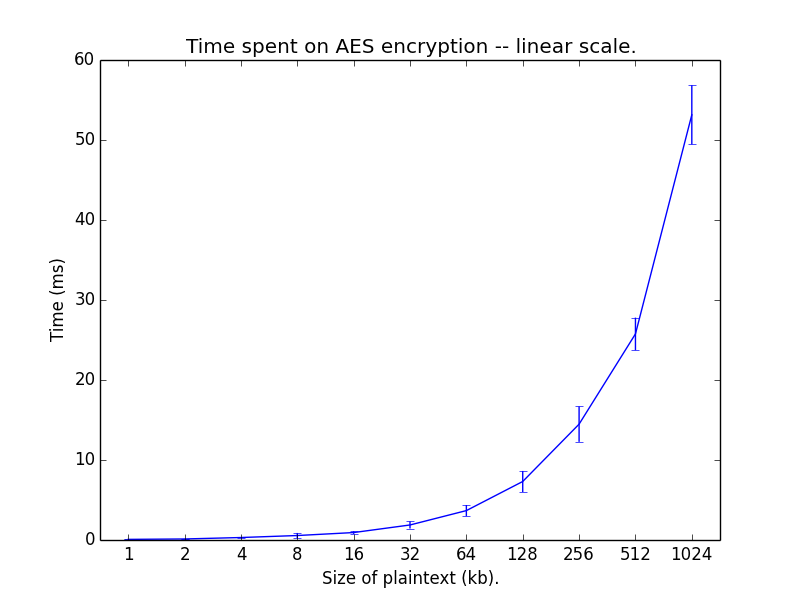
\includegraphics[width=1.1\linewidth]{images/aes_linear}
  \caption{Linear y--scale.}
\end{subfigure}%
\begin{subfigure}{.5\textwidth}
  \centering
  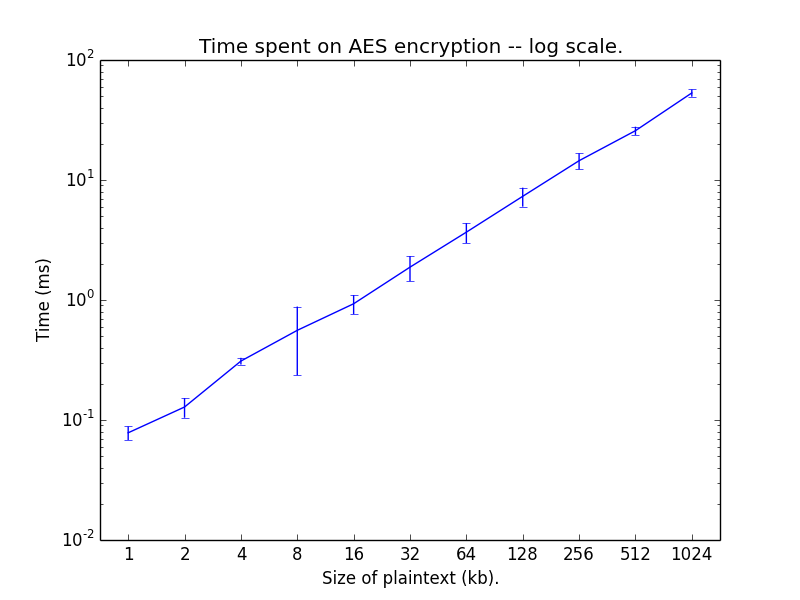
\includegraphics[width=1.1\linewidth]{images/aes_log}
  \caption{Logarithmic y--scale.}
\end{subfigure}
\caption{Time spent in client on \myref{AES}.}
\label{fig:aes}
\end{figure}

As we can see, the results support our expectations, given the linear nature of the curve, in the log--scale graph.
Moreover, with minor exceptions, the time variance seems to be proportional on all levels of data size.
This shows that the library has a consistent and reliable behavior.
Also, even at roughly 100 mb files, the encryption step would still take less than 60ms, which is still considerably less than browser page load times (order of seconds), for example.
Thus, application responsiveness would not be particularly bottlenecked on the time spent on security aspects, inside Nigori.
